\documentclass[twocolumns]{IEEEtran}%twoside, lettersize, onecolumn]{IEEEtran}

\usepackage[
    markup=default,
    authormarkup=none,
    draft
]{changes}

%%% PACKAGES FROM AUTHORS
\usepackage{amsmath, amssymb, tikz, enumitem, tabularx, bm, amsthm, mathabx, import, subfiles, subfigure, mathtools, tikz-cd, xfrac, dsfont, authblk, xr, lineno, xcolor, tikz-3dplot}

% put in the preamble -------------------------------------------------
\usepackage{marginnote}
\newif\ifshowlabels         % master switch

\showlabelstrue             % ← draft
%q\showlabelsfalse            % ← final

\newcommand{\revlbl}[1]{%
  \ifshowlabels
    \marginnote{\footnotesize\color{purple}{\textup{[#1]}}}%
  \fi}
% ---------------------------------------------------------------- ----

%\linenumbers

%%% THEOREM AND LEMMA STRUCTURES

\newtheorem{proposition}{Proposition}
\newtheorem{lemma}[proposition]{Lemma}
\newtheorem{conjecture}[proposition]{Conjecture}
\newtheorem{theorem}[proposition]{Theorem}
\newtheorem{hypothesis}[proposition]{Hypothesis}
\newtheorem{corollary}[proposition]{Corollary}
\newtheorem{claim}[proposition]{Claim}

\theoremstyle{definition}
\newtheorem{definition}[proposition]{Definition}
\newtheorem{example}[proposition]{Example}
\newtheorem{remark}[proposition]{Remark}
\newtheorem{notation}[proposition]{Notation}
\newtheorem{speculation}[proposition]{Speculation}

\newcommand{\Z}{\ensuremath{\mathbb{Z}}}% integers
\newcommand{\N}{\ensuremath{\mathbb{N}}}% natural numbers
\newcommand{\R}{\ensuremath{\mathbb{R}}}% real numbers
\newcommand{\C}{\ensuremath{\mathbb{C}}}% complex numbers
\newcommand{\Q}{\ensuremath{\mathbb{Q}}}
\newcommand{\inv}{\ensuremath{^{-1}}}
\newcommand{\mfa}{\ensuremath{\mathfrak{a}}}
\newcommand{\mcO}{\ensuremath{\mathcal{O}}}
\newcommand{\PR}{\ensuremath{\mathbb{P}}}

\newcommand{\cat}[1]{\ensuremath{\bm{\mathrm{#1}}}}
\newcommand{\bmX}{\ensuremath{\bm{X}}}
\newcommand{\bmx}{\ensuremath{\bm{x}}}
\newcommand{\bma}{\ensuremath{\bm{\alpha}}}
\newcommand{\bmb}{\ensuremath{\bm{\beta}}}
\newcommand{\phid}{\ifmmode \Phi\,\mathrm{ID} \else $\Phi\,\mathrm{ID}$ \fi}
\newcommand{\phiwms}{\ensuremath{\Phi^{\text{WMS}}}}
\newcommand{\mcA}{\ensuremath{\mathcal{A}}}
\newcommand{\U}{\ensuremath{\mathcal{U}}}
\newcommand{\Prob}{\ensuremath{\mathbb{P}}}
\newcommand{\Bint}{\ensuremath{B^\circ}}
\newcommand{\Lint}{\ensuremath{\mu}}

\newcommand{\catname}[1]{{\normalfont\textbf{#1}}}
\newcommand{\FinProb}{\catname{FinProb}}
\newcommand{\LintD}{\ensuremath{\frac{\partial \mu}{\partial x}}}

\newcommand\indep{\perp\!\!\!\perp}

\DeclareMathOperator{\Red}{Red}
\DeclareMathOperator{\Syn}{Syn}
\DeclareMathOperator{\Un}{Un}
\DeclareMathOperator{\In}{In}
\DeclareMathOperator{\Dk}{\mathcal{D}^{(k)}}
\DeclareMathOperator{\Gk}{\mathcal{G}^{(k)}}
\DeclareMathOperator{\Sk}{\mathcal{S}^{(k)}}
\DeclareMathOperator{\image}{im}
\DeclareMathOperator{\kurt}{kurt}
\DeclareMathOperator{\Tr}{Trace}
\DeclareMathOperator{\sgn}{sgn}
\DeclareMathOperator{\content}{\mathcal{C}}
\DeclareMathOperator{\Dis}{Dis}
\DeclareMathOperator{\ord}{ord}
\DeclareMathOperator{\Hom}{Hom}
\DeclareMathOperator{\id}{id}
\DeclareMathOperator{\Rep}{Rep}
\DeclareMathOperator{\TC}{TC}
\DeclareMathOperator{\DTC}{DTC}
\DeclareMathOperator*{\Star}{\bigast}
\DeclareMathOperator{\sig}{\textbf{sig}}

\newcommand{\I}{\ensuremath{\mathcal{I}}}
\renewcommand{\phi}{\varphi}
\renewcommand{\epsilon}{\varepsilon}

\newcommand{\dd}{\ensuremath{\mathrm{d}}}

\usetikzlibrary{decorations.markings, shapes, positioning}

%%%%%
%% correct bad hyphenation here
\hyphenation{op-tical net-works semi-conduc-tor}


\usepackage{graphicx} % Required for inserting images

\title{Improving on weighted symbolic mutual information}

\author[1]{Keenan J. A. Down}

\affil[1]{\textit{Independent researcher, Cambridge, United Kingdom}}

\usepackage{subfiles}

\begin{document}

\maketitle

\begin{abstract}
The weighted symbolic mutual information (wSMI), introduced by King et al. in 2013, is a commonly used measure of signal connectivity in MEG and EEG analyses. Derived from the permtutation entropy, wSMI captures interactions between signal patterns across time-series at a specified temporal resolution, but accounts for volume conductivity effects by weighting out perfect instantaneous synchrony or asynchrony. We show that this weighting-out method is mathematically not well-founded, showing that it can lead both to negative mutual information (which should be theoretically impossible) and to potential spurious biases. Using a recently emerging perspective on scaleless information theory, we propose a correction to the weighting procedure for wSMI, creating a new measure, called conditional Symbolic Mutual Information (cSMI). We show that this new measure behaves similarly to wSMI but is mathematically well-founded, unbiased, and straightforward to implement in current wSMI pipelines.
\end{abstract}

\section{Introduction}
% Weighted symbolic MI exists
Weighted symbolic mutual information (wSMI) is a widely-used information measure that is often applied to EEG data in cognitive neuroscience \cite{king2013information, sitt2014large, imperatori2019eeg, gaubert2019eeg, imperatori2021cross, ding2023resting, van2024local, baki2024decision}. Derived from the permutation entropy \cite{bandt2002permutation}, the wSMI accounts for three challenging problems encountered with noisy EEG signals: stability under the presence of noise, non-linear interactions between signals, and accounting for volume conductance effects in EEG \cite{nobody}.

% Old measures are linear.
Early connectivity measures such as functional connectivity \cite{friston1993functional, friston1994functional, biswal1995functional} or EEG coupling \cite{nobody} look at linear correlations and relationships between the time series of two different signals. One way to improve on these measures is to account for interactions which are also non-linear. Information theory, built around the central concepts of entropy and mutual information \cite{shannon1948mathematical}, is one such powerful tool. Information-theoretic connectivity measures capture \textit{all} relationships between signals --- linear and non-linear.

% Noise.
In general, some information measures can be difficult to apply to EEG data, as EEG signals exhibit non-stationarity, despite the frequent and often useful application of Gaussian models \cite{ince2017statistical}. In particular, EEG signal amplitudes can change significantly, meaning that discretisation and binning (one standard method for avoiding the Gaussian assumption) can lead to unusual results. To get around this, permutation entropy and wSMI look at the \textit{shapes} of signals, coding them by a simplified representation (the symbol) which is invariant to amplitude \cite{bandt2002permutation, king2013information}.

% Volume conduction
Finally, and most importantly for our examination here, the wSMI, like the weighted Phase Lag Index (wPLI), attempts to circumvent a particular problem with EEG: the instantaneous conduction of signal, not necessarily representative of actual brain activity or connectivity \cite{nobody}. For the wSMI, this involves \textit{weighting} certain combinations of symbol pairs (which volume conduction might generate) so as to discount them \cite{king2013information, imperatori2019eeg}. This weighting, however, introduces a slight mathematical complication. In particular, while mutual information is mathematically destined to be non-negative \cite{shannon1948mathematical}, weighting the probabilities in this fashion breaks this property \cite{imperatori2019eeg, kvaalseth1991relative}.

\section{Weighted Symbolic Divergence}

We introduce a new measure, the \textbf{weighted symbolic divergence}.

\begin{definition}
Let $S$ denote the set of retained symbol pairs after filtering out volume conduction pairs, and define
\[
m = \sum_{(i,j)\in S} p_{XY}(i,j),
\qquad
z = \sum_{(i,j)\in S} p_X(i)p_Y(j).
\]
Then
\[
\operatorname{wSD}(\pi_X;\pi_Y)
=
m\,D_{\mathrm{KL}}\!\left(
\frac{p_{XY}|_S}{m}
\;\middle\|\;
\frac{(p_Xp_Y)|_S}{z}
\right),
\]
where $p_X$ and $p_Y$ are the original, unmasked marginals.
When $m=0$, define $\operatorname{wSD}(\pi_X;\pi_Y)=0$.
\end{definition}

\begin{figure}[h]
\centering
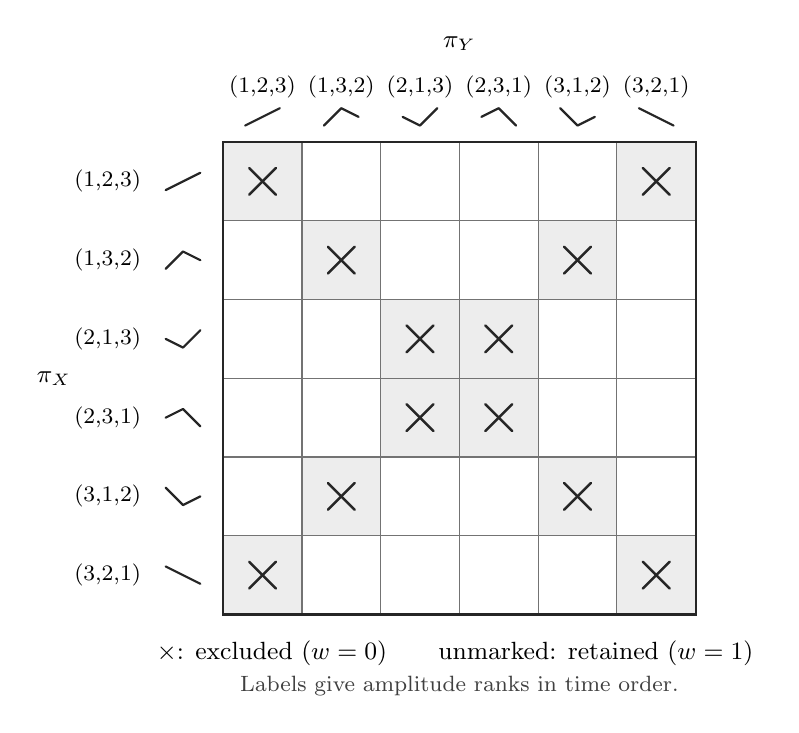
\begin{tikzpicture}[
    x=1cm, y=1cm,
    font=\small,
    pattern/.style={draw=black!85, line width=0.8pt, line cap=round,
                    line join=round},
    cross/.style={draw=black!85, line width=0.9pt, line cap=round}
]

% Shade excluded cells and draw the crosses.
\foreach \row in {1,...,6} {
    \foreach \col in {1,...,6} {
        \pgfmathtruncatemacro{\excluded}{
            (\row == \col) || (\row + \col == 7)
        }
        \ifnum\excluded=1\relax
            \fill[black!7] (\col-1,6-\row) rectangle (\col,7-\row);
            \draw[cross] (\col-0.67,6.33-\row)
                       -- (\col-0.33,6.67-\row);
            \draw[cross] (\col-0.67,6.67-\row)
                       -- (\col-0.33,6.33-\row);
        \fi
    }
}

% Six-by-six grid.
\draw[step=1, draw=black!55, line width=0.45pt] (0,0) grid (6,6);
\draw[draw=black!85, line width=0.8pt] (0,0) rectangle (6,6);

% Permutation labels and miniature ordinal patterns on both axes.
\foreach \i/\a/\b/\c in {
    1/1/2/3, 2/1/3/2, 3/2/1/3,
    4/2/3/1, 5/3/1/2, 6/3/2/1
} {
    % Column label and pattern: signal Y.
    \node[font=\footnotesize] at (\i-0.5,6.70) {$(\a,\!\b,\!\c)$};
    \draw[pattern] (\i-0.72,{6.10+0.11*\a})
                -- (\i-0.50,{6.10+0.11*\b})
                -- (\i-0.28,{6.10+0.11*\c});

    % Row label and pattern: signal X.
    \node[anchor=east, font=\footnotesize] at (-0.92,6.5-\i)
        {$(\a,\!\b,\!\c)$};
    \draw[pattern] (-0.73,{6.5-\i+0.11*(\a-2)})
                -- (-0.51,{6.5-\i+0.11*(\b-2)})
                -- (-0.29,{6.5-\i+0.11*(\c-2)});
}

\node at (3,7.25) {$\pi_Y$};
\node at (-2.15,3) {$\pi_X$};

% Optional legend: remove these nodes when supplying a separate caption.
\node[align=center] at (3,-0.49) {
    $\times$: excluded ($w=0$)\qquad unmarked: retained ($w=1$)
};
\node[font=\footnotesize, text=black!75] at (3,-0.91) {
    Labels give amplitude ranks in time order.
};
\end{tikzpicture}
\caption{The outcomes available from wSMI. The crossed sections indicated are removed in the calculation in order to account for volume conduction.}
\end{figure}


\section{Validation on sample data}
% Here's a toy system with negative wSMI.
% Wow in wSD it's positive how nice.
% Here's an experimental system with a problem.
% Here's how it looks now.

\section{Conclusion}

In this manuscript we introduced weighted symbolic divergence (wSD) as a potential successor to the weighted symbolic mutual information (wSMI). We demonstrated that where the wSMI is not always a positive quantity, wSD has the useful property that it is strictly positive for all possible distributions, while still accounting for the volume conduction effects that wSMI was designed to handle.

Not only this, we saw that the wSD proposed has many natural and intuitive properties. It is bounded above by the raw mutual information between the two permutation variables, behaves locally like mutual information away from the weighted-out volume conduction nodes, and is intuitively familiar to the construction of mutual information as a KL-divergence.

In our analysis we also demonstrated that this new measure, wSD, is well behaved both on toy systems and experimental data: it is straightforward to calculate and exhibits behaviour familiar to wSMI while strengthening its mathematical foundations.

We expect there may be other weighted information quantities which have similar symmetry-breaking behaviour beyond the wSMI. We believe that applying a similar rescaling procedure and using the KL-divergence will be a natural way to apply this method in many different domains.

\bibliographystyle{plain}
\bibliography{main.bib}

\end{document}
